% !Mode:: "TeX:UTF-8:Main"
% arara: pdflatex
% arara: convert: {density: 160, otheroptions: -dispose previous -delay 60 -loop 0, format: gif}
% xarara: showfile: {format: gif}
\documentclass{article}
\usepackage[utf8]{inputenc} %probably not needed ...
\usepackage[T1]{fontenc}
\usepackage{geometry}
\geometry{papersize={128mm,96mm},margin=0.5cm} %\textwidth=11.8, \textheight=8.6
\usepackage[x11names,svgnames]{xcolor}
\usepackage{tikzducks}
\usepackage{scsnowman}
\usepackage{tikzpeople,eso-pic,tikzlings,xfp}
\usetikzlibrary{shadings}
\pagestyle{empty} %cat hippo panda pig rhino
\parindent=0pt
\definecolor{pskin}{RGB}{255,200,184}%
\definecolor{phair}{RGB}{249,249,139}%
\definecolor{mggreen}{RGB}{37,166,89}
\tikzset{
   90iduck/.pic = {
   \begin{scope}[scale=0.8,transform shape]
     \hippo;
  \end{scope}},
   180iduck/.pic = {
   \begin{scope}[scale=0.8,transform shape]
     \cat;
  \end{scope}},
   270iduck/.pic = {
   \begin{scope}[scale=0.8,transform shape]
     \pig;
  \end{scope}},
   0iduck/.pic = {
   \begin{scope}[scale=0.8,transform shape]
     \bear;
  \end{scope}},
  210duck/.pic = {
   \begin{scope}[scale=0.8,transform shape]
     \marmot;
  \end{scope}},
  30duck/.pic = {
   \begin{scope}[scale=0.8,transform shape]
    \rhino;
  \end{scope}},
 60duck/.pic =
  {
   \begin{scope}[scale=0.8,transform shape]
   \owl;
   \end{scope}},
 90duck/.pic =
  {
   \begin{scope}[scale=0.8,transform shape]
   \moles;
   \end{scope}},
  120duck/.pic=
   {
    \begin{scope}[scale=0.8,transform shape]
    \coati;
   \end{scope}
  },
   150duck/.pic=
   {
    \begin{scope}[scale=0.8,transform shape]
    \panda %\duck[santa=red!80!black, jacket=red!80!gray, tshirt=white,beard=white!80!brown,body=LightGoldenrod2!70!RosyBrown1]
    \end{scope}
    },
  180duck/.pic=
  {
   \begin{scope}[scale=0.8,transform shape]
   \koala;
   \end{scope}
  },
  330duck/.pic=
  {
   \begin{scope}[xshift=-0.8cm,scale=0.8,transform shape]
    \begin{scope}[xshift=-0.2cm,scale=0.3,overlay]
    \fill[white]
     plot[variable=\x,domain=0:360,samples=72]
     ({4.8+\x/90},{6.75+0.2*cos(\x/(1+abs(0.1*(10))))})
     --
     plot[variable=\x,domain=0:360,samples=72]
    ({4.8+(360-\x)/90},{4.75+0.2*cos((360-\x)/(1+abs(0.1*(10))))})
    --cycle;
    \fill[red]
     plot[variable=\x,domain=0:360,samples=72]
     ({4.8+\x/90},{5.90+0.2*cos(\x/(1+abs(0.1*(10))))})
     --
     plot[variable=\x,domain=0:360,samples=72]
    ({4.8+(360-\x)/90},{5.60+0.2*cos((360-\x)/(1+abs(0.1*(10))))})
     -- cycle;
     \fill[red]
     plot[variable=\x,domain=160:200,samples=72]
     ({4.8+\x/90},{6.75+0.2*cos(\x/(1+abs(0.1*(10))))})
    --
    plot[variable=\x,domain=160:200,samples=72]
   ({4.8+(360-\x)/90},{4.75+0.2*cos((360-\x)/(1+abs(0.1*(10))))})
    -- cycle;
     \fill[left color=gray, right color=gray,middle color=gray!50!white] ([xshift=-1mm]4.8,7.0)--++ (0,-4.8)--++(2mm,0)--++(0,4.8)--cycle;
   \end{scope}
   \duck
   \end{scope}
  },
  240duck/.pic= {
   \begin{scope}[scale=0.75,transform shape]
   \mouse\end{scope}} ,
  270duck/.pic= {\begin{scope}[scale=0.8,transform shape]\snowman;\end{scope}} ,
  300duck/.pic =
   {
   \begin{scope}[scale=0.8,transform shape]
  \penguin
    \end{scope}
   },
   0duck/.pic = {\begin{scope}[scale=0.8,transform shape]
  \sloth
    \end{scope}},
  }



\colorlet{treecolor}{LawnGreen!50!black}
\tikzset{tree/.pic={
    \begin{scope}[scale=0.2]	
    \filldraw[brown] (-.5,-.5) rectangle ++(1,1.5);
	\filldraw[treecolor] (0,1)
	to[bend right] ++(4,0)
	to[bend left] ++(-3,2)
	to[bend right] ++(2,0)
	to[bend left] ++(-2.5,2)
	to[bend right] ++(1,0)
	to[bend left] ++(-1.5,2)
	-- cycle;
	\filldraw[treecolor] (0,1)
	to[bend left] ++(-4,0)
	to[bend right] ++(3,2)
	to[bend left] ++(-2,0)
	to[bend right] ++(2.5,2)
	to[bend left] ++(-1,0)
	to[bend right] ++(1.5,2)
	-- cycle;
	\begin{scope}[shift={(-.6,6.4)}, scale=.6]
		\duck
	\end{scope}
    \end{scope}}
}
\begin{document}
\AddToShipoutPictureBG{%
 \AtPageLowerLeft{%
 \begin{tikzpicture}[overlay,remember picture]
 \node[anchor=center] at (current page.center)%{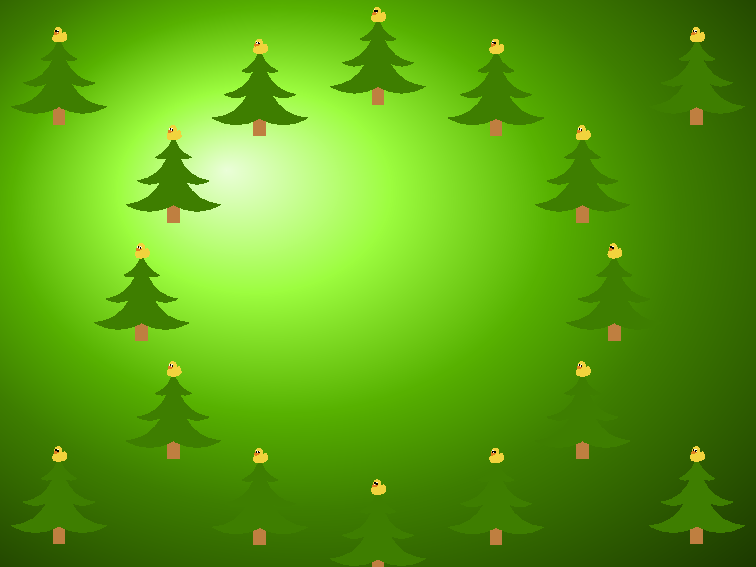
\includegraphics[width=\fpeval{1.2+\value{page}*0.007}\paperwidth]{trees}};
 {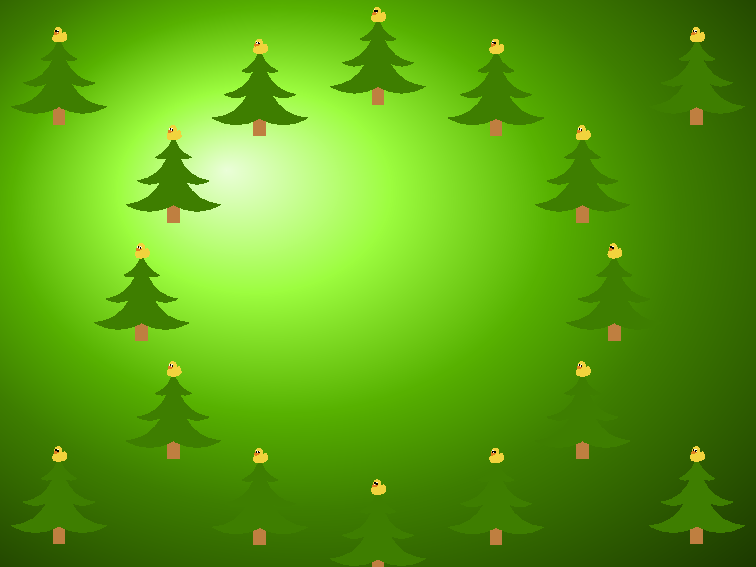
\includegraphics{trees}};
 %\shade[ball color=LawnGreen] (0,0) rectangle (\paperwidth,\paperheight);
% \path ([xshift=1cm,yshift=-2cm]current page.north west) pic {tree};
% \path ([xshift=1cm,yshift=0.5cm]current page.south west) pic {tree};
% \path ([xshift=-1cm,yshift=-2cm]current page.north east) pic {tree};
% \path ([xshift=-1cm,yshift=0.5cm]current page.south east) pic {tree};
 \end{tikzpicture}}}
\foreach \x in {0,2,...,360} %355 {0,10,...,80}%
{%
\begin{tikzpicture}

\path (0,0) rectangle (\textwidth,\textheight);
%\begin{scope}[xshift=50mm,yshift=35mm,overlay]
%\duck[body=pskin!80!white,longhair=phair,tshirt=magenta!60!white,jacket=magenta!40!white,
%necklace=white!85!yellow]
%\fill[yellow!80!orange,rotate=-10,xshift=-11,yshift
%=5] \duckpathcrown;
%
\coordinate (mycenter) at (0.5\textwidth,0.4\textheight);
%%\draw ([yshift=0.2cm,xshift=0.2cm]wing) circle (3cm);
%\end{scope}

  \foreach \y in {0,30,...,330}%
 {
  \path[overlay] (mycenter) --+(\x+\y:3.5) pic { \y duck };
 }

 \foreach \y in {0,90,180,270}%
 {
  \path[overlay] (mycenter) --+(\x+\y:1.5) pic { \y iduck };
 }

%\draw(0,0)--(mycenter);
\end{tikzpicture}\newpage
}
\end{document} 